\documentclass[
	12pt,				% tamanho da fonte
	openright,			% capítulos começam em pág ímpar (insere página vazia caso preciso)
	oneside,			
	a4paper,			% tamanho do papel
	chapter=TITLE,		% títulos de capítulos convertidos em letras maiúsculas
	section=TITLE,		% títulos de seções convertidos em letras maiúsculas
	%subsection=TITLE,	% títulos de subseções convertidos em letras maiúsculas
	%subsubsection=TITLE,% títulos de subsubseções convertidos em letras maiúsculas
	% -- opções do pacote babel --
	english,			% idioma adicional para hifenização
	brazil,				% o último idioma é o principal do documento
	]{abntex2}

\usepackage{udesc}

\usepackage{float} % para forçar a posição das figuras

% Para fazer marcações:
\usepackage{color}
\usepackage{ulem}
\newcommand\hl{\bgroup\markoverwith
  {\textcolor{yellow}{\rule[-.5ex]{2pt}{2.5ex}}}\ULon}

% Para desenhar (autômatos, e.g.):
\usepackage{tikz}
\usetikzlibrary{automata, positioning, arrows}
\tikzset{
    node distance=3cm,
    every state/.style={semithick},
    double distance=2pt,
    every edge/.style={
        draw,
        ->,>=stealth',
        auto,
        semithick
    },
    initial text=$ $
}

\usepackage{amsthm}
\newtheorem{teo}{Teorema}
\newtheorem{lem}{Lema}

\usepackage{amsmath}

\usepackage{amssymb} % para usar o símbolo de conjunto vazio

% Para determinar o número da última página na Ficha Catalográfica:
\usepackage{lastpage}

% Para agilizar a inserção de figuras:
\newcommand{\figura}[4]{
	\begin{figure}[H]
    	\caption{#1}
    	\begin{center}
        	#2
    	\end{center}
    	\legend{Fonte: #4.}
    	\label{#3}
    \end{figure}
}
\newcommand{\figuradoautor}[3]{
    \figura{#1}{#2}{#3}{Elaborada pelo autor, 2019}
}
\def\arraystretch{1.3}
\usepackage{multirow}
\newcommand{\novoquadro}[4]{
	\begin{quadro}[H]
		\footnotesize
		\caption{#1}
		\label{#3}
		\centering
		#2
		\legend{Fonte: #4.}
	\end{quadro}
}
\newcommand{\quadrodoautor}[3]{
	\novoquadro{#1}{#2}{#3}{Elaborado pelo autor, 2019}
}

% Dados da capa:
\titulo{Especificação e prova de propriedade acerca de autômatos finitos determinísticos assistidas por Coq}
\autor{Filipe Ramos}
\local{Joinville - SC}
\instituicao{Universidade do Estado de Santa Catarina - Udesc}
\campus{Centro de Ciências Tecnológicas - CCT}
\curso{Bacharelado em Ciência da Computação}
\data{2019}
\fulldata{xx de xxxx de 2019}

% Dados da folha de rosto:
\inforosto{Trabalho de Conclusão de Curso apresentado ao curso de Bacharelado em Ciência da Computação como requisito parcial para a obtenção do título de Bacharel em Ciência da Computação.}
\orientador{Karina Girardi Roggia}
\orientadorRotulo{Dra. }
\coorientador{Rafael Castro Gonçalves Silva}
\coorientadorRotulo{Me. }

\begin{document}

%!TEX root = ../Principal.tex
% Capa do trabalho:
\imprimircapa


% Folha de rosto:
%* indica que tem ficha catalográfica
\imprimirfolhaderosto*


% Caso a Biblioteca da UDESC forneça, utilize o comando
% \begin{fichacatalografica}
%     \includepdf{fig_ficha_catalografica.pdf}
% \end{fichacatalografica}

% Geração da ficha catalográfica via LaTeX:
%\begin{fichacatalografica}
%	\vspace*{\fill}					% Posição vertical
%	\begin{center}					% Minipage Centralizado
%	\begin{minipage}[c]{12.5cm}		% Largura
%	
%	\imprimirautor
%	
%	\hspace{0.5cm} \imprimirtitulo  / \imprimirautor. --
%	\imprimirlocal, \imprimirdata-
%	
%	\hspace{0.5cm} \pageref{LastPage} p. : il. (algumas color.) ; 30 cm.\\
%	
%	\hspace{0.5cm} \imprimirorientadorRotulo~\imprimirorientador\\
%	
%	\hspace{0.5cm}
%	\parbox[t]{\textwidth}{\imprimirtipotrabalho~--~\imprimirinstituicao,
%	\imprimirdata.}\\
%	
%	\hspace{0.5cm}
%		1. Tópico 01.
%		2. Tópico 02.
%		I. Prof. Dr. xxxxx.
%		II. Universidade do Estado de Santa Catarina.
%		III. Centro de Educação do Planalto Norte.
%		IV. identificação xxxx\\ 			
%	
%	\hspace{8.75cm} CDU 02:121:005.7\\
%	
%	\end{minipage}
%	\end{center}
%\end{fichacatalografica}


% Folha de aprovação:
% Exemplo de folha de aprovação antes da Banca. Após isso, incluia o pdf digitalizado com as assinaturas%
% \includepdf{folhadeaprovacao_final.pdf}
%\begin{folhadeaprovacao}
%
%	\begin{center}
%		{\ABNTEXchapterfont\bfseries\imprimirautor}
%		\vspace{6em}
%
%			\ABNTEXchapterfont\bfseries\imprimirtitulo
%		
%	\end{center}
%		\vspace{1em}
%		{\justify
%		Trabalho de Conclusão de Curso apresentado ao curso de Bacharelado em Ciência da Computação como requisito parcial para a obtenção do título de Bacharel em Ciência da Computação}
%	
%	\vspace{3em} 
%	\noindent
%	{\bfseries Banca examinadora:}
%	\assinatura{\textbf{Dra. Karina Girardi Roggia} \\ Universidade do Estado de Santa Catarina (Udesc)} 
%	\assinatura{\textbf{Dr. Cristiano Damiani Vasconcellos} \\ Udesc}
%    \assinatura{\textbf{Dr. Roberto Silvio Ubertino Rosso Junior} \\ Udesc}
%
%%    \vspace*{\fill}
%    \begin{center}
%    	\imprimirlocal,\,\imprimirfulldata
%    \end{center}
%\end{folhadeaprovacao}


% Dedicatória:
%\begin{dedicatoria}				
%Dedico este trabalho a...  
%\end{dedicatoria}


% Agradecimentos:
%\begin{agradecimentos}
%Gostaria de agradecer...

%Aqui devem ser colocadas os agradecimentos às pessoas que de alguma forma contribuíram para a realização do trabalho.
%\end{agradecimentos}


% Epígrafe:
%\begin{epigrafe}	
%``frase''
%\\
%\par
%autor
%\end{epigrafe}


% Resumo em português:
\begin{resumo}
    RESUMO AQUI

    \vspace{\onelineskip}
    
    \noindent
    \textbf{Palavras-chaves}: .
\end{resumo}


% Resumo em inglês:
\begin{resumo}[Abstract]
    \begin{otherlanguage*}{english}
    ABSTRACT
    
    \vspace{\onelineskip}
    
    \noindent 
    \textbf{Keywords}: .
    \end{otherlanguage*}
\end{resumo}


% Lista de figuras:
\pdfbookmark[0]{\listfigurename}{lof}
\listoffigures*
\cleardoublepage


% Lista de tabelas:
% \pdfbookmark[0]{\listtablename}{lot}
% \listoftables*
% \cleardoublepage


% Lista de quadros:
\pdfbookmark[0]{\listofquadrosname}{loq}
\listofquadros*
\cleardoublepage
 % texto dos elementos pré-textuais

% Lista de abreviaturas e siglas:
\begin{siglas}
    \acro{AFD}{Autômato finito determinístico}
    \acro{CCI}{Cálculo de construções indutivas}
    \acro{SED}{Sistema a eventos discretos}
    \acro{VANT}{Veículo aéreo não tripulado}
\end{siglas}

% Lista de símbolos:
%\begin{simbolos}
%	\SingleSpacing
%	\item[\%] Porcentagem
%	\item[$D_{ab}$] Distância Euclidiana
%	\item[$O(n)$] Ordem de um algoritmo
%\end{simbolos}

% Sumário:
\pdfbookmark[0]{\contentsname}{toc}
\tableofcontents*
\cleardoublepage

\textual

% Retira o nome do capítulo do header:
\pagestyle{eudesc}
\aliaspagestyle{chapter}{eudesc}


% Texto principal do TCC:
\chapter{Introdução}

Os autômatos são modelos de máquinas abstratas muito importantes para os estudos da computação teórica. Em particular, os autômatos finitos determinísticos (\acs{AFD}s) reconhecem as linguagens regulares, aplicadas na ciência da computação e tecnologia da informação \cite{hopcroft}. Sob outra perspectiva, essa classe de autômatos tem sido utilizada para descrever sistemas do mundo hodierno na automação de indústrias e tecnologias, já que o advento dos sistemas a eventos discretos (\acs{SED}s) impôs um novo paradigma, contrário aos sistemas orientados pelo tempo, que são, em geral, muito bem descritos pelos modelos físicos clássicos e modernos \cite{cassandras}.

Com a finalidade de descrever o funcionamento dos sistemas que são orientados a eventos discretos e assíncronos, eles podem ser modelados por formalismos da matemática discreta, entre os quais podemos citar os autômatos determinísticos, redes de Petri, \textit{timed models} e cadeias de Markov. São exemplos de SEDs que podem ser representados por esses modelos os sistemas de filas, computacionais, de comunicação, manufatura, tráfego, banco de dados e telefonia. Os sistemas de filas, geralmente, envolvem a sincronização de processos manipulando filas ou \textit{buffers}, problema presente na automação industrial. É possível modelar diferentes SEDs com as características dos sistemas de filas a fim de representar plantas industriais com recursos compartilhados entre suas partes. Os AFDs são amplamente usados nesse sentido, já que reduzem o tempo do projeto desses sistemas, permitem formalizá-los e torna mais fácil a manutenção deles \cite{rosso1}.

A obtenção de propriedades sobre AFDs específicos pode não ser uma tarefa trivial, e sua formalização, a prova, costuma mostrar-se ainda mais difícil, pois a intuição, muitas vezes, é o único meio utilizado para a garantia das propriedades. Outra técnica utilizada a fim disso é o \textit{model checking}, no qual os instrumentos de verificação -- \textit{model checkers} -- operam enumerando exaustivamente o espaço dos estados de um modelo. O método é limitante, porque resulta em uma explosão combinatorial, tornando impraticável a verificação de modelos de sistemas reais desse modo \cite{athalye}. Por isso, o emprego de assistentes interativos de provas matemáticas é útil, eles possibilitam a formulação e demonstração das propriedades. Tais assistentes reúnem meios formais e computacionais que propiciam a verificação dos passos da demonstração, auferindo rigor. Entre os assistentes de provas, o Coq destaca-se por ter comunidade extensa, ter uma linguagem funcional de alta ordem e permitir a construção de tipos dependentes. Outras qualidades desse assistente são a possibilidade de programar táticas de provas, desenvolver e carregar módulos separadamente sem a necessidade de verificá-los novamente e definir notações para melhorar a visualização das definições e provas \cite{manualcoq}. O Coq tem se mostrado uma ferramente robusta e bastante aceita pela comunidade acadêmica. O teorema das quatro cores, segundo o qual qualquer mapa pode ser colorido com quatro cores de modo que as regiões adjacentes tenham cores diferentes, foi provado em Coq por \citeonline{4cores}, resultando em uma prova mais rigorosa em relação às demais demonstrações para o mesmo teorema. Embora o computador tenha sido empregado nas outras provas, essa última destaca-se por dispensar a necessidade de confiar nos programas verificadores de casos particulares e ser expressa na confiável linguagem formal do Coq. Essas e outras características do Coq motivaram a escolha dele para a assistência das provas que este trabalho externa.

Os problemas envolvendo filas em processos concorrentes são muito estudados na ciência da computação e dotados de relevância no que tange aos sistemas de produção industrial, onde a falta de sincronização acarreta eventualmente outros problemas. Se um SED é corretamente modelado por AFDs, devemos ser capazes de identificar nos modelos as eventuais falhas decorrentes da concorrência por recursos distribuídos em filas; senão, apontar os defeitos da representação. Por esse motivo, confere-se valor e importância ao presente estudo.

O objetivo geral deste trabalho de conclusão de curso consiste em provar, mediante o assistente de provas Coq, propriedades sobre sistemas da automação industrial modelados por AFDs. Os objetivos específicos são: \begin{enumerate}
	\item introduzir os principais conceitos relativos aos SEDs;
	\item apresentar a classe de sistemas de filas;
	\item especificar propriedades desejadas para essa classe;
	\item empregar o assistente Coq na prova de teoremas referentes a essas propriedades;
	\item demonstrar e explanar tais teoremas e exemplificar sua aplicação.
\end{enumerate}

Com a finalidade de atingir os objetivos supracitados, o presente trabalho é estruturados destarte. Primeiramente, no capítulo \ref{cap:relacionados}, apresentam-se os trabalhos relacionados a este estudo. O capítulo \ref{cap:provas} introduz uma breve noção sobre assistentes de provas e o Coq. No capítulo \ref{cap:seds}, são introduzidos os SEDs, assim como sua modelagem por AFDs. O capítulo seguinte, \ref{cap:filas}, apresenta os sistemas de filas, problemas relacionados e as propriedades mais importantes acerca desses SEDs. Em seguida, o capítulo \ref{cap:propriedades} demonstra como constatar se sistemas de filas atendem às propriedades. Por fim, são expressas as considerações finais e, depois, as referências bibliográficas.
\chapter{Assistentes de provas}
\label{cap:provas}

Um assistente de provas interativo é um artifício de software que auxilia no processo de prova matemática. Diferentemente dos provadores automáticos de teoremas, os assistentes não realizam provas automaticamente com um simples comando do usuário, mas participa com ele no processo oferecendo uma variedade de procedimentos formalizadores. Seu uso também se justifica na necessidade de validar demonstrações, haja vista que detalhes podem passar despercebidos pelo olhar analítico do ser humano. Os assistentes mais robustos implementam a teoria dos tipos, na qual os elementos pertencem a tipos definidos recursivamente, e não a conjuntos.

A teoria dos tipos fornece o encontro da ciência da computação com a matemática e a lógica. Ela é simultaneamente um sistema formal e linguagem de programação que permite raciocinar enquanto se programa. Sua relevância se explica por possuir simplicidade, ser robusta, apresentar a propriedade da decidibilidade, ser uma linguagem funcional, entre outros \cite{luo}.

A Seção \ref{sec:coq} introduz o assistente de provas empregado neste trabalho de conclusão de curso. A escolha do Coq se deve à confiabilidade, utilidade, usabilidade e facilidade desse assistente.

\section{Coq}
\label{sec:coq}

Coq é um dos assistentes de provas mais utilizados atualmente, permitindo a construção de tipos dependentes e polimórficos, lógica de alta ordem, etc. A linguagem formal deste assistente de provas é o cálculo de construções indutivas (\acs{CCI}), no qual há duas variedades de objetos, os tipos e os termos. Os tipos são classes a que pertencem os termos -- o número $1$ é um termo do tipo natural -- e podem ser termos de outros tipos. Nessa linguagem formal, a notação para um termo $x$ do tipo $X$ é $x:X$, com a qual devemos nos habituar para utilizar o Coq \cite{manualcoq}.

No Coq os tipos são definidos indutivamente pelos comandos \texttt{Inductive}, \texttt{Fixpoint} e \texttt{Record}. O primeiro permite definir termos destarte: \begin{align*}
&\texttt{Inductive $ident$ : $term$ :=}\\ &\texttt{$ident_1$ : $term_1$ | $ident_2$ : $term_2$ | $...$ | $ident_n$ : $term_n$.}
\end{align*} em que $ident$ é o nome do objeto sendo definido e $term$ é seu tipo. Cada $ident_i$ e $term_i$ são os respectivos nome e tipo do $i$-ésimo construtor ($\forall i=1..n$). O comando \texttt{Fixpoint} define funções de forma recursiva baseada nos $m$ argumentos: \begin{align*}
&\texttt{Fixpoint $ident$ ($ident_1$ : $term_1$) ($ident_1$ : $term_1$) $...$ ($ident_m$ : $term_m$)}\\&\texttt{: $term$ := $term'$.}
\end{align*} A definição usando esse comando deve garantir que a recursão sempre para. Para tanto, o usuário precisa especificar a recursão mediante a estrutura \texttt{match with}: \begin{align*}
term' := \text{} & \texttt{match $ident_1$, $ident_2$, $...$, $ident_m$ with}\\
& \texttt{$a_1^1$, $a_2^1$, $...$, $a_m^1$ => $term_1'$ |}\\
& \texttt{$a_1^2$, $a_2^2$, $...$, $a_m^2$ => $term_2'$ |}\\
& \vdots\\
& \texttt{$a_1^k$, $a_2^k$, $...$, $a_m^k$ => $term_k'$}\\
& \texttt{end}
\end{align*} Quando não é necessário haver recursão, pode-se substituir o comando \texttt{Fixpoint} pelo \texttt{Definition}. Já o comando \texttt{Record} aproxima o usuário das linguagens de programação comuns, ao definir estruturas parecidas com as quais desenvolvemos nelas: \begin{align*}
&\texttt{Record $ident$ $params$ : $term$ := $ident_0$ \{}\\
&\texttt{$ident_1$ : $term_1$;}\\
&\texttt{$ident_2$ : $term_2$;}\\
&\vdots\\
&\texttt{$ident_n$ : $term_n$ \}.}
\end{align*} em que $params$, $ident_0$, $ident_i$ e $term_i$ são, respectivamente, os parâmetros ou argumentos, nome do construtor (opcional), nome e tipo do $i$-ésimo campo ($\forall i = 1..n$), havendo $n$ campos. Na linguagem do Coq, o $i$-ésimo campo de um \textit{record} é obtido com esta sintaxe: \texttt{$ident_i$ $x$}, em que $x : ident$. Há outras maneiras de definir termos a partir desses comandos, mas as apresentadas são suficientes para os objetivos do presente trabalho.

A sintaxe que visualizamos é a combinação do CCI com a linguagem de especificação Gallina, bastante intuitivos. Para provar teoremas e lemas no Coq, além de definir os tipos que usaremos nas proposições, é necessário utilizar o comando \texttt{Theorem} ou \texttt{Lemma}: $$\texttt{Theorem $ident$ := $ident'$. Proof. $tactic_1$. $tactic_2$. $...$. $tactic_m$. Qed.}$$ com $m$ táticas. As táticas são o cerne da interatividade do Coq e facilitam o desenvolvimento de provas. Elas implementam um raciocínio que parte da conclusão para as premissas, denominadas objetivo e subobjetivos respectivamente. Uma tática, aplicada corretamente sobre o objeto, gera subobjetivos que o substituem \cite{manualcoq}. O Quadro \ref{quad:taticas_coq} apresenta as principais táticas do Coq utilizadas por este trabalho.

\novoquadro{Principais táticas do Coq}{
	\begin{tabular}{|c|c|}
		\hline \textbf{Nome} & \textbf{Descrição}\\ \hline
		\texttt{intros} & Introduz variáveis\\ \hline
		\texttt{simpl} & Simplifica expressão\\ \hline
		\texttt{reflexivity} & Valida expressões $a = a$\\ \hline
		\texttt{rewrite} & Reescreve relações de igualdade\\ \hline
		\texttt{apply} & Aplica um lema, teorema ou axioma\\ \hline
		\texttt{symmetry} & Troca $a = b$ por $b = a$\\ \hline
		\texttt{injection} & Infere $a = b$ a partir de $f(a) = f(b)$, sendo $f$ injetora\\ \hline
		\multirow{2}{*}{\texttt{omega}} & Completa prova a partir de igualdades e\\
		& desigualdades envolvendo inteiros\\ \hline
		\texttt{induction} & Faz indução sobre uma variável\\ \hline
	\end{tabular}
}{quad:taticas_coq}{Elaborado pelo autor com base em \citeonline{manualcoq}, 2019}

Outras táticas importantes são: \texttt{unfold} -- para expandir expressões reduzidas --, \texttt{discriminate} -- usada quando os elementos de uma igualdade são construídos diferentemente, como $1 = 0$ -- e \texttt{inversion}. Esta última faz o Coq analisar outras condições para que uma hipótese seja verdadeira. A fim de exemplificar o uso das táticas do Coq, provemos o teorema $$\texttt{Theorem plus\_n\_O : $\forall$ n : nat, n = n + 0.}$$ em que $nat$ é o tipo dos números naturais. Comecemos removendo o quantificador universal e introduzindo a variável \texttt{n}: $$\texttt{Proof. intros n.}$$ Agora, iniciemos a indução sobre \texttt{n}: $$\texttt{induction n as [|n' IHn'].}$$ em que os símbolos após o ``\texttt{|}'' nomeiam as variáveis a serem utilizadas no passo indutivo. Para a base $\texttt{n} = \texttt{0}$, basta simplificar e aplicar a tática \texttt{reflexivity}. Como esta já simplifica a expressão, não é necessário aplicar \texttt{simpl}. No passo indutivo, temos $\texttt{n} = \texttt{S n'}$, sendo \texttt{S x} a função sucessor de $\texttt{x} : \texttt{nat}$. O objetivo atual é $$\texttt{S n' = S n' + 0}$$ Simplificando com \texttt{simpl}, obtemos $$\texttt{S n' = S (n' + 0)}$$ Agora podemos aplicar a hipótese de indução $\texttt{IHn'} = \texttt{(n' = n' + 0)}$ mediante a tática $$\texttt{rewrite <- IHn'.}$$ com \texttt{<-} indicando que o lado direito da hipótese \texttt{IHn'} deve ser reescrito pelo esquerdo no objetivo, o que gera $$\texttt{S n' = S n'}$$ Por fim, $$\texttt{reflexivity. Qed.}$$ como queríamos demonstrar.

O capítulo seguinte, \ref{cap:seds}, conceitua os sistemas a eventos discretos e autômatos finitos determinísticos, objetos das demonstrações do Capítulo \ref{cap:propriedades}. Essas provas foram obtidas e validadas no ambiente do assistente Coq.
\chapter{Sistemas a eventos discretos}
\label{cap:seds}

Segundo \citeonline[p. 142, tradução do autor]{lafortune} \begin{citacao} Sistemas a eventos discretos (\acs{SED}s) são sistemas dinâmicos com duas características definidoras: seus espaços de estados são discretos e potencialmente infinitos, e sua dinâmica é orientada a eventos, em vez de tempo. (...) Eventos que ocorrem de forma assíncrona (em geral) causam um salto no espaço de estados, de um estado para outro. \end{citacao} \citeonline{cassandras} argumentam que os SEDs, diferentemente dos sistemas orientados pelo tempo e governados pelas leis da natureza, não podem ser modelados e estudados usando equações diferenciais. Os SEDs requerem outras técnicas de análise, ferramentas de projeto, métodos de teste, entre outros.

O advento das tecnologias de comunicação, sensoriamento e computação impulsionou a caracterização desta nova classe de sistemas. Os SEDs, por não serem adequadamente modelados pelas equações das leis da física clássica e moderna, demandam novos paradigmas de modelagem. ``Intuitivamente, nós podemos pensar em um modelo como um dispositivo que simplesmente duplica o comportamento do próprio sistema'' \cite[p. 3, tradução do autor]{cassandras}. Um modelo descreve um sistema sob uma ótica quantitativa, que é, muitas vezes, mais adequada que uma simples e subjetiva descrição qualitativa. A construção de um modelo considera um conjunto de variáveis de entrada e saída, relacionadas por intermédio de uma função. Assim sendo, os modelos proporcionam a habilidade predizer os comportamentos de sistemas, o que os confere importância. Formas de modelar sistemas que evoluem com base em eventos assíncronos e discretos são discutidas neste capítulo.

\citeonline{cassandras} citam, como exemplos de SEDs, os sistemas de filas, computacionais, de comunicação, de manufatura e de tráfego. A exemplo disso, protocolos de comunicação em redes de computadores são frequentemente modelados por SEDs, como indica a Figura \ref{fig:protocolo_rede}. O presente trabalho enfoca os sistemas relacionados à automação industrial, para os quais a modelagem de filas é conveniente. A espera de entidades por um recurso em uma fábrica é exemplo que justifica isso, porque a abstração por meio de filas ou \textit{buffers} é muito útil nesse caso. O capítulo \ref{cap:filas} explanará essa e outras situações em que podemos abstrair a noção de filas.

\figura{Protocolo para um canal de redes de computadores com erros de bits: lado remetente e (abaixo) destinatário}{
	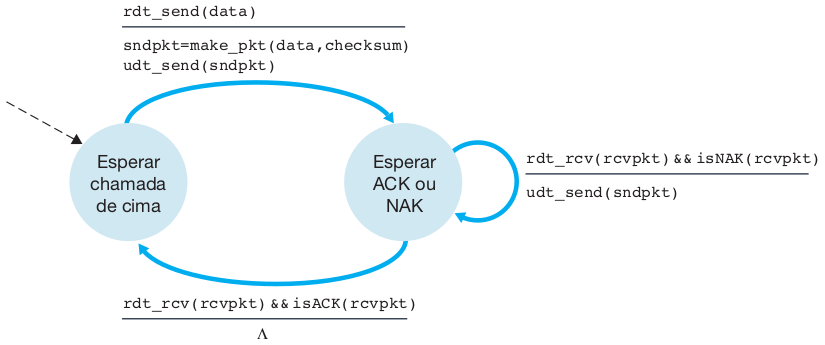
\includegraphics[width=.9 \textwidth]{figuras/rdt2_0-remetente.png}\\
	\vspace{8mm}
	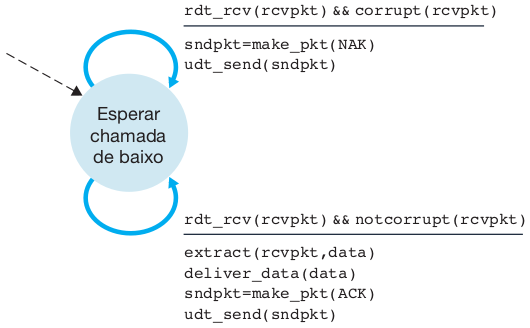
\includegraphics[width=.6 \textwidth]{figuras/rdt2_0-destinatario.png}
}{fig:protocolo_rede}{KUROSE, J.; ROSS K. \textbf{Redes de computadores e a internet}: uma abordagem top-down. 6. ed. São Paulo: Pearson, 2013}

Na figura \ref{fig:protocolo_rede}, tem-se representado um protocolo de redes em que há estados de espera e transições que dependem de eventos discretos -- neste caso, procedimentos computacionais. A representação supracitada é uma evidência do caráter de SED do protocolo, e a figura é um diagrama de estados, que será introduzido mais adiante.

SEDs são comumente modelados por redes de Petri e autômatos determinísticos. Redes de Petri são uma classe de grafos direcionados que têm duas variedades de nós: posições e transições. Nelas, os arcos podem ligar dois nós apenas se forem diferentes -- não pode haver arcos entre duas posições, por exemplo -- e têm pesos que indicam a quantidade de tokens que serão consumidos ou produzidos. Geralmente, os tokens, posições e transições representam recursos, condições e eventos respectivamente e permitem modelar atividades paralelas, protocolos de comunicação, sistemas de produtor-consumidor com prioridade, etc. \cite{petrinets} Este trabalho de conclusão de concurso, todavia, tem enfoque na representação por autômatos finitos determinísticos. A seção \ref{sec:afd}, que segue, introduz os principais conceitos desses modelos.

\section{Autômatos finitos determinísticos}
\label{sec:afd}

Autômato -- palavra derivada do termo em latim \textit{automatu} -- é ``maquinismo que se move por meios mecânicos'' e ``imita os movimentos humanos'' \cite[p. 81]{aurelio}. Esse termo tem sido usado na ciência da computação desde a década de 1930 para descrever importantes modelos da Teoria dos Autômatos, que aborda máquinas de Turing, por exemplo. Nesse contexto, um autômato é uma máquina abstrata descrita matematicamente e idealizada em termos de limitações físicas \cite{hopcroft}.

Um autômato finito determinístico (\acs{AFD}), ou máquina de estados finitos determinística, é uma máquina dotada de fita, unidade de controle e função de transição. A fita de um autômato é um espaço ilimitado utilizado para armazenar uma sequência de símbolos que serão lidos e computados. Já a unidade de controle contém as variáveis do estado atual da máquina, que servem de parâmetro para a computação da função de transição. Para determinar o estado de um autômato, há uma cabeça de leitura sobre a fita e um conjunto de elementos abstratos que norteiam a evolução do funcionamento da máquina: os estados \cite{hopcroft}. A Figura \ref{fig:afd_componentes} esquematiza a transição de estado de um AFD com a cabeça de leitura inicialmente posicionada sobre a segunda célula da fita.

\figuradoautor{Transição de um AFD}{
    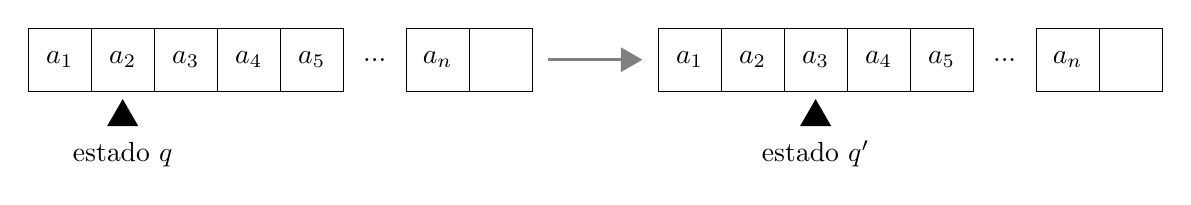
\begin{tikzpicture}
        \draw[draw=black] (0,0.8) rectangle ++(0.8,0.8)
        (0.8,0.8) rectangle ++(0.8,0.8)
        (1.6,0.8) rectangle ++(0.8,0.8)
        (2.4,0.8) rectangle ++(0.8,0.8)
        (3.2,0.8) rectangle ++(0.8,0.8)
        (4.8,0.8) rectangle ++(0.8,0.8)
        (5.6,0.8) rectangle ++(0.8,0.8);
        \draw[>=triangle 60,->,line width=0.6mm] (1.2,0.4) -- (1.2,0.7);
        \node at (1.2,0) {estado $q$};
        \node at (0.4,1.2) {$a_1$};
        \node at (1.2,1.2) {$a_2$};
        \node at (2.0,1.2) {$a_3$};
        \node at (2.8,1.2) {$a_4$};
        \node at (3.6,1.2) {$a_5$};
        \node at (4.4,1.2) {$...$};
        \node at (5.2,1.2) {$a_n$};
        
        \draw[>=triangle 60,->,line width=0.4mm, draw=gray] (6.6,1.2) -- (7.8,1.2);
        
        \draw[draw=black] (8,0.8) rectangle ++(0.8,0.8)
        (8.8,0.8) rectangle ++(0.8,0.8)
        (9.6,0.8) rectangle ++(0.8,0.8)
        (10.4,0.8) rectangle ++(0.8,0.8)
        (11.2,0.8) rectangle ++(0.8,0.8)
        (12.8,0.8) rectangle ++(0.8,0.8)
        (13.6,0.8) rectangle ++(0.8,0.8);
        \draw[>=triangle 60,->,line width=0.6mm] (10.0,0.4) -- (10.0,0.7);
        \node at (10.0,0) {estado $q'$};
        \node at (8.4,1.2) {$a_1$};
        \node at (9.2,1.2) {$a_2$};
        \node at (10.0,1.2) {$a_3$};
        \node at (10.8,1.2) {$a_4$};
        \node at (11.6,1.2) {$a_5$};
        \node at (12.4,1.2) {$...$};
        \node at (13.2,1.2) {$a_n$};
    \end{tikzpicture}
}{fig:afd_componentes}

Durante a computação de uma cadeia de entrada, o AFD lê o símbolo da célula atual da fita, apontada pela cabeça de leitura, e avança o cabeçote em uma posição para a direita. Inicialmente, ao receber uma entrada, a cabeça de leitura estará posicionada na extremidade esquerda da fita e, por conseguinte, da cadeia de símbolos. Se a computação de um símbolo lido não acarretar um estado definido ou a cabeça de leitura estiver posicionada sobre uma célula vazia, o funcionamento do autômato será interrompido.

Na Ciência da Computação, os AFDs formam a base de alguns componentes de software e partes de compiladores. Um artifício muito empregado no desenvolvimento de software são as expressões regulares, que podem ser convertidas em AFDs e permitem encontrar padrões em textos \cite{hopcroft}. Já no contexto dos \acs{SED}s, os AFDs são modelos matemáticos que descrevem sistemas com base nos eventos que podem ocorrer. Dessa maneira, as cadeias de símbolos que são enviadas à entrada dos AFDs constituem sequências de eventos cuja computação resulta em uma descrição do sistema baseada nas variáveis de controle da máquina de estados \cite{cassandras}.

\subsection{Definição formal}

A definição de \acs{AFD} que segue foi inspirada e adaptada de \citeonline{hopcroft} e \citeonline{cassandras}.

Um AFD $G$ é uma quíntupla \begin{equation}
\label{eq:afd}
\langle Q, E, \delta, q_0, Q_m \rangle
\end{equation} em que \begin{itemize}[label={}]
  \item $Q$ é o conjunto finito de estados
  \item $E$ é o conjunto finito de símbolos ou eventos
  \item $\delta:Q \times E \nrightarrow Q$ é a função de transição
  \item $q_0 $ é o estado inicial
  \item $Q_m \subseteq Q$ é o conjunto de estados marcados
\end{itemize}

A função de eventos ativos de $G$, que será denotada por $\Gamma_G:Q \to 2^E$, relaciona cada estado com os eventos possíveis a partir dele. Formalmente, para todo estado $q \in Q$ $$\forall e \in E, e \in \Gamma_G(q) \Leftrightarrow \delta(q, e) \in Q$$ isto é, $e \in \Gamma_G(q)$ se e somente se $\delta(q, e)$ é definido.

Ao fecho de Kleene sobre um conjunto de eventos $E$, denotado por $E^\star$, pertencem todas as possíveis cadeias de eventos pertencentes a $E$. Uma cadeia de eventos é uma sequência finita $e_1 e_2 ... e_{|w|}$ em que $e_i \in E$ ($\forall i = 1..|w|$). Quando $|w| = 0$, a cadeia é dita vazia e será simbolizada por $\varepsilon$.

A função de transição estendida $\hat{\delta}:Q \times E^\star \nrightarrow Q$ é definida recursivamente destarte: $$\hat{\delta}(q, w) = \begin{cases}
q & \text{se $w=\varepsilon$} \\
\hat{\delta}(\delta(q, e), w') & \text{se $w=e w'$}
\end{cases}$$ e terá valor indefinido quando $\delta(q, e)$ assim for.

Embora a formulação matemática de um AFD seja muito útil e importante para formalizar SEDs e provar propriedades destes, a visualização do funcionamento destes autômatos é facilitada com a representação por diagramas de estados. Ademais, tendo em vista que o presente trabalho dispõe de diversos destes diagramas, a subseção seguinte, \ref{subsec:diagramas}, introduz essas representações.

\subsection{Diagrama de estados}
\label{subsec:diagramas}

Para auxiliar na visualização das transições entre os estados dos autômatos, os AFDs são comumente representados por diagramas de estados. Nessa representação, os estados são nós de uma estrutura semelhante a de grafos, e as transições, arestas que interligam dois nós, conforme a Figura \ref{fig:afd_diagrama}. Representam-se as transições cuja origem e destino são o mesmo estado por \textit{loops}: arestas que partem de um nó e terminam no mesmo.

\figuradoautor{Representação da transição de estados em um diagrama}{
    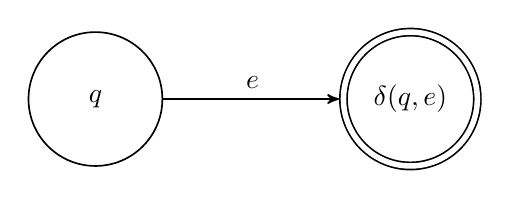
\begin{tikzpicture}[shorten >=1pt,node distance=2cm,on grid,auto] 
        \node[state,minimum size=1.7cm] (q0) {$q$}; 
        \node[state,accepting,minimum size=1.7cm] at (4,0) (q1) {$\delta(q, e)$};
        \draw
        (q0) edge node{$e$} (q1);
    \end{tikzpicture}
}{fig:afd_diagrama}

Nesta classe de diagramas, os estados inicial e final podem ser destacados de alguma forma. Para este trabalho, uma seta sem origem aponta sempre para o nó do estado inicial, e uma circunferência dupla enfatiza o de um estado final, como demonstra a Figura \ref{fig:afd_estado_inicial}.

\figuradoautor{Representação de estados inicial (à esquerda) e final (à direita) em um diagrama}{
    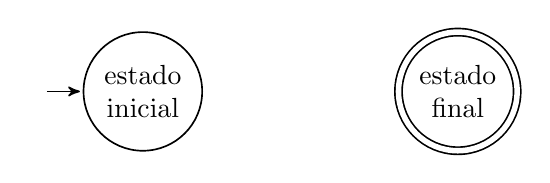
\begin{tikzpicture}[shorten >=1pt,node distance=2cm,on grid,auto] 
        \node[align=center,state,initial] (q0) {estado\\inicial};
        \node[align=center,state,accepting] at (4,0) (qf) {estado\\final};
    \end{tikzpicture}
}{fig:afd_estado_inicial}

Pode-se citar outros aspectos desta representação de autômatos: a possibilidade de adicionar rótulos aos nós, a opção de omitir os nomes dos estados nos nós quando não forem necessários e a aglutinação de transições que partem e terminam no mesmo estado em uma mesma aresta, com os símbolos separados por vírgula.

\subsection{Linguagem marcada}

A linguagem marcada por um AFD $G$ é o conjunto $$L_m(G) = \{ w \in E^\star \mid \hat{\delta}(q_0, w) \in Q_m \}$$ Sendo assim, a linguagem marcada pelo autômato são todas as cadeias de eventos que o fazem transicionar do estado inicial a um estado marcado. Isso significa que, quando uma cadeia $w \in L_m(G)$ for posicionada na fita do autômato, a computação de cada evento, da esquerda para a direita da sequência, sempre resultará em um estado definido e terminará em um estado marcado.

Denomina-se linguagem regular a linguagem marcada por qualquer AFD \cite{hopcroft}. Desse modo, este trabalho de conclusão de curso versará sobre linguagens exclusivamente regulares, a exemplo das quais é possível citar o conjunto dos números naturais pares. Sabendo que um número par é aquele cujo último algarismo -- da esquerda para a direita -- pertence a $\{ 0, 2, 4, 6, 8 \}$, pode-se construir o AFD da Figura \ref{fig:afd_pares}, demonstrando a validade da afirmação.

\figuradoautor{Diagrama de estados para um AFD que reconhece os números naturais pares}{
    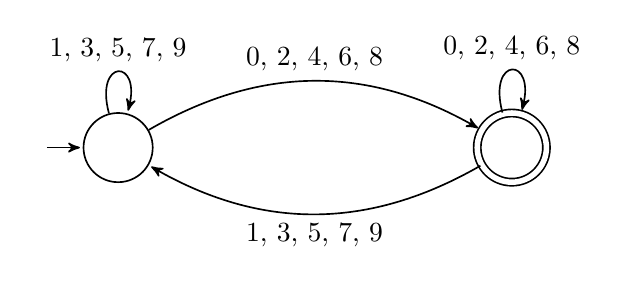
\begin{tikzpicture}[shorten >=1pt,node distance=2cm,on grid,auto] 
        \node[state,initial] (q0) {}; 
        \node[state,accepting] at (5,0) (q1) {};
        \draw
            (q0) edge[loop above] node{$1$, $3$, $5$, $7$, $9$} (q0)
            (q0) edge[bend left, above] node{$0$, $2$, $4$, $6$, $8$} (q1)
            (q1) edge[loop above] node{$0$, $2$, $4$, $6$, $8$} (q1)
            (q1) edge[bend left, below] node{$1$, $3$, $5$, $7$, $9$} (q0);
    \end{tikzpicture}
}{fig:afd_pares}

Quando um autômato se destina a verificar padrões em cadeias de eventos, ou palavras, diz-se que ele é um formalismo reconhecedor \cite{menezes} e, portanto, o autômato da Figura \ref{fig:afd_pares} reconhece todos os números naturais pares. No que tange aos \acs{SED}s, alcançar um estado marcado implica a conclusão de alguma tarefa \cite{cassandras}. A impossibilidade de concluir tarefas, os bloqueios ocorrem quando não é possível sair de um estado não marcado e chegar a um marcado, tema da subseção seguinte, \ref{subsec:ling_ger}.

\subsection{Linguagem gerada e bloqueios}
\label{subsec:ling_ger}

A linguagem gerada por um AFD $G$ é o conjunto $$L(G) = \{ w \in E^\star \mid \hat{\delta}(q_0, w) \in Q \}$$ Neste caso, a linguagem são todas as cadeias de eventos que fazem o autômato transicionar do estado inicial a um estado definido.

Caso o autômato $G$ chegue a um estado $q \not\in Q_m$ tal que $\Gamma_G(q) = \varnothing$, diz-se que há um \textit{deadlock}, já que não existe evento que pode ser executado a partir de $q$. Um \textit{livelock} se configura quando, mesmo não havendo \textit{deadlock}, não é possível alcançar um estado marcado. Se qualquer bloqueio acontece $$\overline{L_m(G)} \subset L(G)$$ em que $\overline{L_m(G)}$ é o conjunto de todos os prefixos de todas as cadeias pertencentes a $L_m(G)$, ou $$\overline{L_m(G)} = \{ w \in E^\star \mid \exists w' \in E^\star, w w' \in L_m(G) \}$$ Isso é devido à constatação de que, tendo sido executada uma cadeia de eventos $w \in E^\star$ e estando em um bloqueio, $w$ pertencerá a $L(G)$, mas não será prefixo de alguma cadeia da linguagem marcada: não haverá $w' \in E^\star$ tal que $ww' \in L_m(G)$, por definição \cite{cassandras}.

\subsection{Função de transição total}

Haja vista que não é possível formular funções parciais no assistente de provas Coq, algumas mudanças na definição de AFD supracitada são necessárias a fim de representar AFDs nessa ferramenta. A começar, é impreterível alterar a função de transição de um AFD $G$ para torná-la total. Seja $\delta' : Q \cup \{ \otimes \} \times E \to Q \cup \{ \otimes \}$ a seguinte função total: $$\delta'(q, e) = \begin{cases}
\delta(q, e) & \text{se $\delta(q, e) \in Q$} \\
\otimes & \text{senão}
\end{cases}$$ em que $\otimes$ é um estado novo, não pertencente a $Q$: o estado de ralo.

O autômato $G$ é muito semelhante ao $$G' = \langle Q \cup \{ \otimes \}, E, \delta', q_0, Q_m \rangle$$ uma vez que a única diferença entre eles é que, em $G'$, ao realizar-se uma transição que seria indefinida em $G$, alcança-se um estado do qual não se pode sair.

Como a função $\delta'$ é total, tem-se que $$L(G') = E^\star$$ em termos do que se estabeleceu como linguagem gerada anteriormente. Pode-se, não obstante, modificar a definição dela de forma que $G$ e $G'$ sejam equivalentes em se tratando de linguagens: \begin{equation}
\label{eq:ling_ralo}
L'(G') = \{ w \in E^\star \mid \hat{\delta}(q_0, w) \in Q \wedge \hat{\delta}(q_0, w) \neq \otimes \}
\end{equation} é a linguagem gerada pelo autômato $G'$. Então $$L'(G') = L'(G) = L(G)$$

É possível visualizar as formulações de um AFD usando função de transição parcial e total na Figura \ref{fig:afd_funcao_total}, que a exemplifica para um AFD de alfabeto $\{ a, b \}$.

\figuradoautor{Um AFD simples (à esquerda) e seu correspondente com função de transição total (à direita)}{
	\raisebox{-0.5\height}{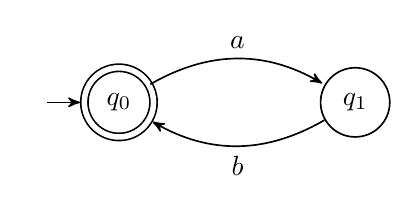
\begin{tikzpicture}[shorten >=1pt,node distance=2cm,on grid,auto] 
	\node[state,initial,accepting] (q0) {$q_0$}; 
	\node[state] at (3,0) (q1) {$q_1$};
	\draw
	(q0) edge[bend left, above] node{$a$} (q1)
	(q1) edge[bend left, below] node{$b$} (q0);
	\end{tikzpicture}}
	\raisebox{-0.5\height}{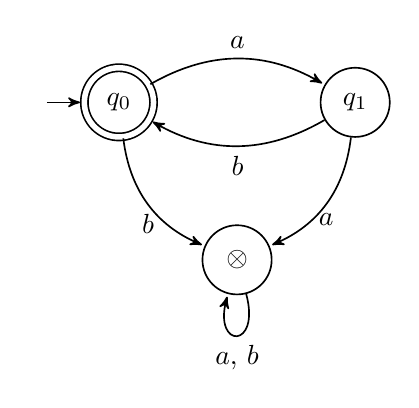
\begin{tikzpicture}[shorten >=1pt,node distance=2cm,on grid,auto] 
	\node[state,initial,accepting] at (0, 2) (q0) {$q_0$}; 
	\node[state] at (3,2) (q1) {$q_1$};
	\node[state] at (1.5,0) (q2) {$\otimes$};
	\draw
	(q0) edge[bend left, above] node{$a$} (q1)
	(q0) edge[bend right, below] node{$b$} (q2)
	(q1) edge[bend left, below] node{$a$} (q2)
	(q1) edge[bend left, below] node{$b$} (q0)
	(q2) edge[loop below] node{$a$, $b$} (q2);
	\end{tikzpicture}}
}{fig:afd_funcao_total}

Isso posto, é evidente que um AFD cuja função de transição não é total pode ser modelado matematicamente utilizando funções totais. Esse fato é importante para que se possa representá-lo na linguagem do Coq.

\subsection{Formulação em Coq}
\label{subsec:afd_coq}

Todas as definições acerca de AFDs supracitadas utilizam conjuntos, mas, para representar os autômatos no assistente de provas Coq, é necessário que sejam usados tipos. Assim, estados e eventos terão tipos específicos.

Conforme a subseção 3.1.5, a formulação de AFDs em Coq precisa considerar o estado de ralo para que a função de transição seja sempre total. Nesse sentido, pode-se definir os estados como do seguinte tipo paramétrico: $$\text{\texttt{Inductive state \{Q : Type\} := sink\_state | proper\_state (q : Q).}}$$ sendo \textit{proper state} -- estado próprio -- qualquer estado do autômato exceto o de ralo. Ao invés de usar apenas o tipo \texttt{Q}, essa definição é importante para facilitar a caracterização das linguagens geradas, já que o estado de ralo tem de estar bem delimitado para defini-las, como demonstra a equação \ref{eq:ling_ralo}.

A função de transição será do tipo \texttt{Q$\to$E$\to$state}, e não \texttt{state$\to$E$\to$state}, o que permitiria quaisquer transições partindo do estado de ralo. Ademais, é importante especificar quais estados são marcados com uma função do tipo \texttt{Q$\to$bool} que retorna \texttt{true} se e somente se o estado for marcado.

Com isso, um autômato determinístico \texttt{g : dfa} terá estes campos: \begin{itemize}
	\item \texttt{Q}: o tipo dos estados próprios
	\item \texttt{E}: o tipo dos símbolos ou eventos
	\item  \texttt{transition : Q$\to$E$\to$@state Q}: a função de transição
	\item \texttt{initial\_state : Q}: o estado inicial
	\item \texttt{is\_marked : Q$\to$bool}: a função de demarcação dos estados
\end{itemize}

Esta definição permite que termos do tipo \texttt{dfa} sejam, com efeito, autômatos infinitos determinísticos. O presente trabalho, porém, assume que os tipos dos estados e eventos são sempre finitos. A implementação do tipo \texttt{dfa} proposta é apresentada pela Figura \ref{fig:dfa_record}.

\figuradoautor{Implementação do tipo dos AFDs em Coq}{
	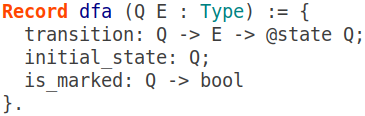
\includegraphics[width=8cm]{figuras/dfa_record.png}
}{fig:dfa_record}

A definição de AFD anterior é equivalente a esta. Sejam $q_1$, $q_2$, $...$ e $q_n$, $q^*$ e $e_1$, $e_2$, $...$ e $e_m$, respectivamente, todos os estados, o estado inicial e todos os possíveis símbolos de um AFD, podemos construir os tipos que seguem: \begin{gather*}\texttt{Inductive Q := $q_1$ | $q_2$ | $...$ | $q_n$.}\\ \texttt{Inductive E := $e_1$ | $e_2$ | $...$ | $e_m$.}\end{gather*} que são os respectivos tipos dos estados e eventos do autômato na definição para o Coq. Seja $\delta : \{ q_1, q_2, ..., q_n \} \times \{ e_1, e_2, ..., e_m \} \nrightarrow \{ q_1, q_2, ..., q_n \}$ a função de transição de estados tal que $$\delta(q, e) = \begin{cases}
q' & \text{se \texttt{transition $q$ $e$ $=$ proper\_state $q'$}}
\end{cases}$$ ou, por outro lado, seja \texttt{transition : Q$\to$E$\to$@state Q} assim definida na linguagem do Coq: 	\begin{align*}
&\texttt{Fixpoint transition (q : Q) (e : E) : state :=}\\
&\texttt{match q, e with}\\
&\texttt{$q'$, $e'$ => proper\_state $\delta(q', e')$ |}\\
&\texttt{\_, \_ => sink\_state}\\
&\texttt{end.}
\end{align*} sendo $x = (q',e')$ todo par tal que $\delta(x)$ é definido. Além disso, determinemos o conjunto de estados marcados: $$Q_m = \{ q_i \mid i \in \{ 1, 2, ..., n \} \wedge \texttt{is\_marked $q_i$ $=$ true} \}$$ ou, de outra parte, construamos a função \texttt{is\_marked}: \begin{align*}
&\texttt{Fixpoint is\_marked (q : Q) : bool :=}\\
&\texttt{match q with}\\
&\texttt{$q_m$ => true |}\\
&\texttt{\_ => false}\\
&\texttt{end.}
\end{align*} em que $q_m$ é todo estado pertencente a $Q_m$. Portanto, o autômato $\langle \{ q_1, q_2, ..., q_n \}, \{ e_1, e_2, ..., e_m \}, \delta, q^*, Q_m \rangle$ pode ser formulado em termos dos elementos \texttt{Q}, \texttt{E}, \texttt{transition} e \texttt{is\_marked} e vice-versa.

Toda sequência de eventos será representada por uma lista, e a função de transição estendida \texttt{extended\_transition} será do tipo \texttt{dfa$\to$@state Q$\to$list E$\to$@state Q} e definida recursivamente. Se o estado de origem for o de ralo, ele será o próprio retorno da função; senão, \texttt{extended\_transition} computará a função de transição para a cabeça da lista de eventos e fará recursão destarte: \begin{gather*}
\texttt{extended\_transition g (proper\_state q) [] = proper\_state q;}\\\texttt{extended\_transition g (proper\_state q) e::w =}\\\texttt{extended\_transition g (transition q e) w}\end{gather*}

Por definição, uma lista de eventos \texttt{w} será gerada por \texttt{g}, ou \texttt{g ==> w}, se $$\texttt{extended\_transition g (proper\_state initial\_state) w $\neq$ sink\_state}$$ ou seja, se a computação da função de transição estendida da lista partindo do estado inicial não resultar no estado de ralo, em conformidade com a equação \ref{eq:ling_ralo}. Sendo $G$ o AFD definido conforme a equação \ref{eq:afd} e equivalente ao \texttt{g}, podemos notar $$L(G) = \{ a_1a_2...a_n \in E^\star \mid \texttt{g ==> [$a_1$;$a_2$;$...$;$a_n$]} \}$$ evidenciando também a correlação entre as diferentes definições supracitadas para a mesma classe de máquinas abstratas.

\section{Autômatos finitos não determinísticos}

Um autômato finito não determinístico (\acs{AFND}) é um modelo diferenciado com a capacidade de estar em mais de um estado ao mesmo tempo \cite{hopcroft}. Essa característica configura a predição dessas máquinas abstratas, permitindo estimar os possíveis estados em que um SED se encontra. Para um AFND $G = \langle Q, E, \delta, q_0, Q_m \rangle$, a função de transição é do tipo $\delta : Q \times Q \to 2^Q$, retornando um conjunto de estados.

A função de transição estendida $\hat{\delta} : Q \times E^\star \to 2^Q$ é tal que para todo estado $q \in Q$, cadeia $w \in E^\star$ e evento $e \in E$ $$\hat{\delta}(q, w) = \begin{cases}
\{ q \} & \text{se $w = \varepsilon$}\\
\displaystyle\bigcup_{q' \in \delta(q, e)} \hat{\delta}(q', w') & \text{se $w = ew'$}
\end{cases}$$ Com ela, as linguagens gerada e marcada por um AFND $G$ são respectivamente $$L(G) = \{ w \in E^\star \mid \hat{\delta}(q_0, w) \neq \varnothing \}$$ e $$L_m(G) = \{ w \in E^\star \mid \hat{\delta}(q_0, w) \cap Q_m \neq \varnothing \}$$ isto é, os conjuntos de todas as cadeias de eventos que fazem o autômato transicionar a algum estado qualquer e marcado respectivamente.

A vantagem de empregar AFNDs reside no fato de que a modelagem de SEDs é facilitada. Quando a execução de um evento resulta em diferentes significados, podemos designar a transição levando a um conjunto de estados cujo nome expressa algum resultado. Por exemplo, supondo que um sistema contém três produtores e um sensor que indica a produção de algum item, um jeito de modelar o sistema é por meio de uma máquina abstrata que vai do estado $\langle n_1, n_2, n_3 \rangle$, ao ser executado um evento de produção, para os pertencentes a $\{ \langle n_1+1, n_2, n_3 \rangle, \langle n_1, n_2+1, n_3 \rangle, \langle n_1, n_2, n_3+1 \rangle \}$, em que $n_1$, $n_2$ e $n_3$ são os respectivos números de itens produzidos pelo primeiro, segundo e terceiro agentes.

\citeonline{hopcroft} demonstram a conversão de qualquer AFND $G$ para um AFD $G'$ usando a construção de subconjuntos, de forma que $L(G) = L(G')$ e $L_m(G) = L_m(G')$. Assim, convertendo os modelos, podemos usar os teoremas do capítulo \ref{cap:propriedades} para verificar propriedades de sistemas modelados por AFND.
\chapter{Problemas de filas}

Os sistemas de filas constituem importante classe de sistemas a eventos discretos (\acs{SED}s) em que entidades ou objetos devem esperar para obter um determinado recurso. Há três elementos básicos que compõem esses sistemas: \begin{itemize}
	\item consumidor: entidade que espera por um recurso;
	\item servidor: o recurso que é aguardado;
	\item fila: o espaço em que os consumidores esperam.
\end{itemize} Os recursos são genericamente denominados servidores por geralmente proverem serviço \cite{cassandras}. O presente trabalho aborda uma ótica abstrata dos sistemas de filas, já que há a possibilidade de reduzir problemas a esses sistemas.

Para ser atendido por um servidor de banco, uma pessoa deve esperar em uma fila até que as pessoas a sua frente sejam atendidas. Esse sistema de filas pode ser modelado pelo autômato infinito determinístico ilustrado pela Figura \ref{fig:sist_enfil_simples_infinito}, em que $+$ e $-$ são os respectivos eventos de chegada e partida de pessoa da fila.

\figuradoautor{Um sistema de filas simples}{
	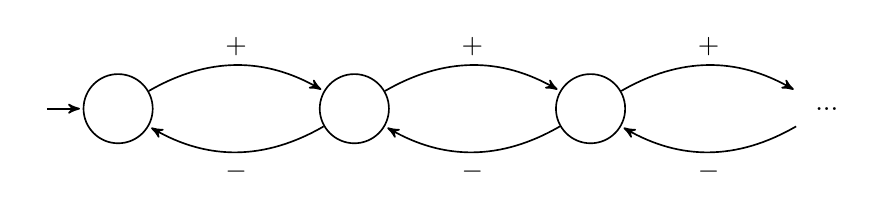
\begin{tikzpicture}[shorten >=1pt,node distance=2cm,on grid,auto] 
		\node[state,initial] (q0) {}; 
		\node[state] at (3,0) (q1) {};
		\node[state] at (6,0) (q2) {};
		\node[state,draw=none] at (9,0) (q3) {$...$};
		\draw
		(q0) edge[bend left, above] node{$+$} (q1)
		(q1) edge[bend left, below] node{$-$} (q0)
		(q1) edge[bend left, above] node{$+$} (q2)
		(q2) edge[bend left, below] node{$-$} (q1)
		(q2) edge[bend left, above] node{$+$} (q3)
		(q3) edge[bend left, below] node{$-$} (q2);
		\end{tikzpicture}
}{fig:fila_simples_infinito}

Na Figura \ref{fig:fila_simples_infinito} é assumido que a fila de pessoas pode crescer indefinidamente, o que não é possível na realidade. Assumindo que as filas têm um tamanho máximo, faz-se possível modelar vários sistemas de filas por meio de autômatos finitos determinísticos (AFDs).

Um exemplo de sistema de filas é apresentado por \citeonline{victor} e consiste em uma planta de fila de demandas para veículos aéreos não tripulados (\acs{VANT}s). Nele as demandas são os consumidores, e os VANTs, os servidores.

\section{Problema do produtor e consumidor}

\section{Propriedades desejadas}

\subsection{Aplicações}

\chapter{Garantia de propriedades em sistemas de filas}

Posto que são desejáveis as constatações de certas propriedades referentes a sistema de filas, um grupo de sistemas a eventos discretos (SEDs), este capítulo visa demonstrar a garantia da existência de capacidade máxima e volume mínimo zero nestes sistemas. Na visão de \citeonline{reisig}, provas acerca de tais propriedades não são completamente triviais, o que evidencia a conveniência auferida com a assistência do provador de teoremas Coq.

Introduzamos algumas notações e definições úteis para nosso propósito. Para representar as operações de adição e retirada de fila, utilizemos os respectivos símbolos $+$ e $-$. Seja $G = \langle Q, E, \delta, q_0, Q_m \rangle$ um autômato finito determinístico (AFD) definido conforme a equação \ref{eq:afd} em que $E \supseteq \{ +, - \}$, queremos provar que o sistema de filas modelado por $G$ satisfaz as duas propriedades supracitadas no capítulo \ref{cap:filas}: que a fila tenha uma capacidade máxima e não seja permitido efetuar operação de retirada de item quando ela estiver vazia.

Precisamos de uma função $c : E^\star \to \mathbb{Z}$ que conte o número de itens armazenados em uma fila após uma cadeia de eventos $w \in E^\star$. Uma forma de defini-la é $$c(w) = \begin{cases}
c(w') + 1 & \text{se $w=+w'$}\\
c(w') - 1 & \text{se $w=-w'$}\\
0 & \text{senão}
\end{cases}$$ Em tal definição, consideramos que o número inicial de itens na fila do sistema é sempre zero. Para sistemas de filas com um número $n_0 \neq 0$ de itens inicialmente dispostos na fila, a quantidade de volume armazenado, após uma cadeia de eventos $w$, será $c(w) + n_0$. Baseado nas propriedades aritméticas da soma de inteiros, podemos observar para quaisquer $w_1$ e $w_2 \in E^\star$ $$c(w_1w_2) = c(w_1) + c(w_2)$$ que será útil para a prova dos teoremas acerca das propriedades dos sistemas de filas.

A fim de facilitar a leitura dos teoremas, simplifiquemos a notação para a transição estendida de um estado $q$ por uma cadeia de eventos $w$ da seguinte maneira: $$qw \equiv \hat{\delta}(q,w)$$ Pelo mesmo motivo, definamos a função $t : E \to \mathbb{Z}$ desta forma: $$t(e) = \begin{cases}
1 & \text{se $e=+$} \\
-1 & \text{se $e=-$} \\
0 & \text{senão}
\end{cases}$$

As seções \ref{sec:capac_max} e \ref{sec:vol_min} apresentam duas condições necessárias e suficientes para que um dado sistema de filas tenha capacidade máxima e volume mínimo zero respectivamente. Para os SEDs com filas que começam com um número $n_0$ de itens alocados nelas, consideremos seu volume inicial igual a zero e a capacidade máxima e volume mínimos subtraídos em $n_0$ unidades, permitindo que os teoremas funcionem para esses casos.

\section{Garantia de capacidade máxima}
\label{sec:capac_max}

O teorema que esta seção aborda surgiu do seguinte questionamento: há algum modo de mapear cada estado do sistema ao número máximo de itens na fila que pode haver naquele estado? Com isso, poderíamos simplesmente verificar o número mapeado por cada estado e obter o maior deles: a capacidade máxima, como desejamos. Há de se salientar que, nos casos de sistemas que permitem um número indefinidamente grande de volume na fila, esse mapeamento não pode existir. Já os sistemas de filas que respeitam a propriedade da capacidade máxima obrigatoriamente permitem o mapeamento.

Obter intuitivamente o mapeamento dos estados para os tamanhos máximos da fila e avaliar seu corretismo pode ser uma tarefa dispendiosa. Verificando um conjunto de regras, não obstante, a atividade torna-se um pouco mais simples. Se um estado $q$ é mapeado por $f : Q \to \mathbb{Z}$ a um número inteiro $m$, qualquer transição partindo de $q$ deve respeitar $$f(qe) \geq m + t(e)$$ para qualquer evento $e \in E$. O teorema \ref{teo:teo1} utiliza essa concepção para exprimir uma condição suficiente para que o SED modelado por $G$ tenha uma capacidade máxima.

\begin{teo}
	\label{teo:teo1}
	Existe uma função $f : Q \to \mathbb{Z}$ e um inteiro $n$ tal que \begin{equation*}
	f(q_0) = 0 \wedge [(\forall q \in Q)(\forall e \in E), f(qe) \geq f(q) + t(e) \wedge f(q) \leq n]
	\end{equation*} se e somente se a fila do sistema modelado por $G$ tem sempre no máximo $n$ itens.
\end{teo}

Devemos demonstrar a validade do teorema. Provemos antes o lema que segue, de utilidade para esse fim.

\begin{lem}
	\label{lem:lema1}
	Para toda função $f : Q \to \mathbb{Z}$, é válido que\begin{equation*}
	\begin{aligned}
	f(q_0) = 0 \wedge [(\forall q \in Q)(\forall e \in E), f(qe) \geq f(q) + t(e)]\\\Rightarrow \forall w \in L(G), c(w) \leq f(q_0w)
	\end{aligned}
	\end{equation*}
\end{lem}
\begin{proof}
A prova deste lema será por indução em $w$, tendo como base $$c(\varepsilon) \leq f(q_0\varepsilon)$$ o que é verdade, pois $c(\varepsilon) = 0$ e é pressuposto $f(q_0) = 0$.

Para o passo indutivo, temos de provar que, para todo evento $u \in E$, se $ wu$ é gerada por $G$, então $$c(wu) = c(w) + t(u) \leq f(q_0wu)$$ ou \begin{equation}
\label{eq:goallema1}
c(w) \leq f(q_0wu) - t(u)
\end{equation} é válido a partir da hipótese de indução.

Sabemos que, se $wu$ é gerada por $G$, então o prefixo $w$ também é. Diante disso \begin{equation}
\label{eq:hipindlema1}
c(w) \leq f(q_0w)
\end{equation} é obtido da hipótese de indução.

Com base na hipótese do lema, obtemos \begin{equation}
\label{eq:hiplema1}
f(q_0w) \leq f(q_0wu) - t(u)
\end{equation}

A partir das equações \ref{eq:hipindlema1} e \ref{eq:hiplema1}, verifica-se $$c(w) \leq f(q_0w) \leq f(q_0wu) - t(u)$$ demonstrando a equação \ref{eq:goallema1}, como queríamos.
\end{proof}

Dado que o presente relatório é apenas parte de um trabalho de conclusão de curso, justifica-se o caráter parcial que assumirá a prova do teorema \ref{teo:teo1}. Nesse sentido, a demonstração que segue é a respeito da condição unidirecional da esquerda para a direita.

\begin{proof}
Aplicando o lema \ref{lem:lema1} na hipótese do teorema, obtemos $$\forall w \in L(G), c(w) \leq f(q_0w)$$

Da hipótese também temos $$f(q_0w) \leq n$$

Portanto $$c(w) \leq f(q_0w) \leq n$$ como desejávamos demonstrar.
\end{proof}

A demonstração do lema 1 e teorema 1 foram auxiliadas pelo Coq, no qual a formulação de AFDs seguiu o exposto na subseção \ref{subsec:afd_coq}. Ao ser transcrita a prova do assistente para este trabalho, as noções de tipos foram trocadas pelas de conjuntos, com a qual estamos habituados na teoria dos autômatos.

Na figura \ref{fig:ex1_teo1}, há um exemplo que ilustra um sistema de produtor e consumidor. Nela os eventos $p$ e $c$ são, respectivamente, a produção e consumo de item. Seja $f_1$ uma função cuja imagem está rotulada nos nós da figura, indicando para cada estado o valor mapeado. Como $f_1$ respeita o teorema \ref{teo:teo1}, podemos concluir que o sistema modelado permite volume máximo de um item na fila.

\figuradoautor{Exemplo de aplicação do teorema \ref{teo:teo1} em um sistema com capacidade máxima $1$}{
	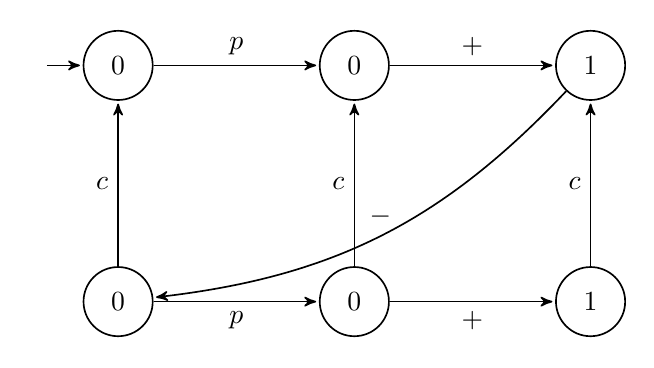
\begin{tikzpicture}[shorten >=1pt,node distance=2cm,on grid,auto] 
	\node[state,initial] (q0) {$0$}; 
	\node[state] at (3,0) (q1) {$0$};
	\node[state] at (6,0) (q2) {$1$};
	\node[state] at (0,-3) (q3) {$0$};
	\node[state] at (3,-3) (q4) {$0$};
	\node[state] at (6,-3) (q5) {$1$};
	\draw
	(q0) edge[above] node{$p$} (q1)
	(q1) edge[above] node{$+$} (q2)
	(q2) edge[above,bend left=20] node{$-$} (q3)
	(q3) edge[below] node{$p$} (q4)
	(q4) edge[below] node{$+$} (q5)
	(q3) edge[left] node{$c$} (q0)
	(q4) edge[left] node{$c$} (q1)
	(q5) edge[left] node{$c$} (q2);
	\end{tikzpicture}
}{fig:ex1_teo1}

Sob outra perspectiva, a figura \ref{fig:ex2_teo1} apresenta um exemplo de AFD modelando um sistema que permite, notavelmente, adição e retirada de um número indefinido de itens da fila. Supondo que tal sistema atenda à propriedade da capacidade máxima, seja $f_2 : \{ q_0, q_1 \} \to \mathbb{Z}$ qualquer função que mapeie cada estado a um número inteiro de forma que $f_2(q_0) = 0$ e $f_2(qe) \geq f_2(q) + t(e)$ para todo evento $e \in \{+,-\}$. É fácil notar que $f_2$ não existe, pois, como $q_1+ = q_1$, podemos obter o absurdo: $f(q_1) \geq f(q_1) + t(+)$. Com isso, o teorema \ref{teo:teo1} conclui que o sistema não admite capacidade máxima.

\figuradoautor{Exemplo de sistema que não tem capacidade máxima definida}{
	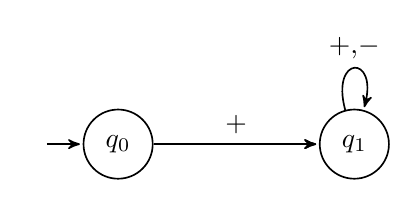
\begin{tikzpicture}[shorten >=1pt,node distance=2cm,on grid,auto] 
	\node[state,initial] (q0) {$q_0$};
	\node[state,initial] at (3,0) (q1) {$q_1$};
	\draw
	(q0) edge node{$+$} (q1)
	(q1) edge[loop above] node{$+$,$-$} (q1);
	\end{tikzpicture}
}{fig:ex2_teo1}

Além de provar que determinados sistemas de filas cumprem ou não com a especificação de uma fila com volume máximo, muitas vezes quer-se atestar a impossibilidade de efetuar operação de retirada de fila vazia. É sobre isso que trata a seção \ref{sec:vol_min}, a seguir.

\section{GARANTIA DE VOLUME MÍNIMO}
\label{sec:vol_min}

Todo sistema de filas especificado com base em \citeonline{cassandras} deve impedir a remoção de itens de filas quando estas forem vazias. Isso é em razão do caráter físico e não abstrato com que se configuram as filas por aquela ótica. Mesmo para filas abstratas, pode ser interessante que esta propriedade seja respeitada. A fim de garantir isso, o teorema \ref{teo:teo2} nos possibilita obter resposta à pergunta: a fila tem volume mínimo de zero itens?

\begin{teo}
	\label{teo:teo2}
	Existe uma função $f : Q \to \mathbb{Z}$ tal que \begin{equation*}
	f(q_0) = 0 \wedge [(\forall q \in Q)(\forall e \in E), f(qe) \leq f(q) + t(e) \wedge f(q) \geq 0]
	\end{equation*} se e somente se a fila do sistema modelado por $G$ nunca tem volume negativo.
\end{teo}

A ideia intuitiva que originou o teorema é semelhante à com que se concebeu o teorema \ref{teo:teo1}. Neste caso, o mapeamento é feito de cada estado $q$ ao número mínimo de itens que podem haver na fila ao se processar qualquer cadeia de eventos fazendo o autômato transicionar de $q_0$ a $q$. Mais uma vez, se é impossível realizar o mapeamento, o sistema não cumpre com a propriedade.

Considerando o autômato da figura \ref{fig:ex1_teo2}, verificamos que o sistema nela representado tem uma fila que respeita esta propriedade, embora não garanta capacidade máxima. Tomando a função $f_3$ rotulada nos nós da figura, pode-se notar que ela respeita o teorema \ref{teo:teo2}, evidenciando que tal SED foi modelado de modo a não permitir o evento $-$ nos momentos em que a fila está vazia.

\figuradoautor{Exemplo de sistema que atende à propriedade de volume mínimo zero}{
	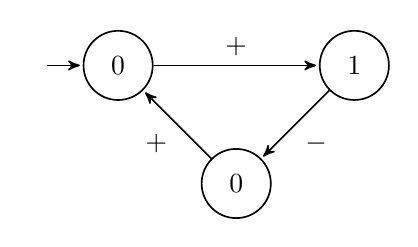
\begin{tikzpicture}[shorten >=1pt,node distance=2cm,on grid,auto] 
	\node[state,initial] (q0) {$0$};
	\node[state] at (3,0) (q1) {$1$};
	\node[state] at (1.5,-1.5) (q2) {$0$};
	\draw
	(q0) edge node{$+$} (q1)
	(q1) edge node{$-$} (q2)
	(q2) edge node{$+$} (q0);
	\end{tikzpicture}
}{fig:ex1_teo2}

Como exemplo de aplicação do teorema \ref{teo:teo2} para um caso de não atendimento a esta propriedade, seja o AFD da figura \ref{fig:ex2_teo2}. Supondo que o sistema satisfaça a restrição de volume mínimo zero, deve haver uma função $f_4 : \{ q_0, q_1, q_2 \} \to \mathbb{Z}$ respeitando $f(q_0) = 0$ e $f_4(qe) \leq f_4(q) + t(e)$ para todo evento $e \in \{+, -\}$. Dessa suposição, obtemos $f_4(q_1) \leq f_4(q_1-) - 1 \leq f_4(q_1--) - 2 \leq f_4(q_1--+) - 1$, um absurdo, uma vez que $q_1--+ = q_1$. Dessarte, o teorema \ref{teo:teo2} implica que, no sistema modelado, há a possibilidade de executar operações de retirada de fila mesmo quando ela está vazia.

\figuradoautor{Exemplo de sistema que permite operações de retirada de fila vazia}{
	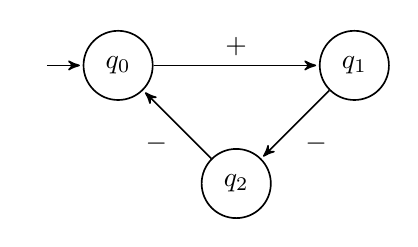
\begin{tikzpicture}[shorten >=1pt,node distance=2cm,on grid,auto] 
	\node[state,initial] (q0) {$q_0$};
	\node[state] at (3,0) (q1) {$q_1$};
	\node[state] at (1.5,-1.5) (q2) {$q_2$};
	\draw
	(q0) edge node{$+$} (q1)
	(q1) edge node{$-$} (q2)
	(q2) edge node{$-$} (q0);
	\end{tikzpicture}
}{fig:ex2_teo2}

Quando aplicamos o teorema \ref{teo:teo2} no autômato da figura \ref{fig:ex1_teo1}, notamos que a própria função rotulada nos nós do diagrama respeita as regras da condição apresentada nesta seção. Em razão desse fato, o tamanho da fila do sistema ilustrado é sempre algum inteiro do intervalo $[0,1]$. Os teoremas deste capítulo também podem ser usados nos exemplos do capítulo \ref{cap:filas} para efeito de demonstração de aplicação.

\chapter{Considerações parciais}
\label{cap:consideracoes}

Este trabalho apresentou os principais conceitos relacionados à modelagem de sistemas a eventos discretos (\acs{SED}s) por meio de autômatos finitos determinísticos (\acs{AFD}s), bem como os relativos a sistemas de filas. As duas restrições do problema do produtor-consumidor foram abordadas, originando métodos formais a fim de garantir as propriedades da capacidade máxima e volume mínimo zero em sistemas de filas. Um teorema foi provado mediante o assistente de provas Coq, enquanto outro será provado na continuação deste trabalho de conclusão de curso.

Como resultado de produção do trabalho, foram escritas 237 linhas de código Gallina na IDE do Coq. O processo passou por uma formalização inicial, que foi simplificada gradativamente. O estado parcial da implementação é uma interface mais bem estruturada e organizada.

Entre as dificuldades encontradas durante a produção deste trabalho, pode-se citar a procura de aplicações realistas de SEDs e sistemas de filas. Os exemplos citados neste trabalho são demasiados simples, não correspondendo a sistemas reais da automação industrial. Outro impasse surgiu nos estudos bibliográficos acerca dos assistentes de provas, uma vez que há muitas teorias que sustentam tais artefatos.

Para a continuidade do presente trabalho, novos teoremas e problemas poderão ser formulados. A generalização dos métodos formais para autômatos finitos não determinísticos também possivelmente será feita, assim como a especificação e verificação de algoritmos de \textit{model-checking} baseados nos teoremas.

Com respeito aos desenvolvimentos feitos no Coq, as formulações e provas relativas aos teoremas expostos neste trabalho encontram-se na página do Github do autor, acessíveis em: $$\text{\href{https://github.com/fil1pe/tcc}{\texttt{https://github.com/fil1pe/tcc}}}$$

% Finaliza o bookmark do PDF:
\bookmarksetup{startatroot}% 

\postextual

% Referências bibliográficas:
\bibliography{referencias}

% Glossário:
%
% Consulte o manual da classe abntex2 para orientações sobre o glossário.
%
%\glossary

% Apêndices:
%\begin{apendicesenv}
%	\include{Partes/apeA}
%\end{apendicesenv}

% Anexos:
%\begin{anexosenv}
%	\include{Partes/aneA}
%\end{anexosenv}

\end{document}

